\documentclass{beamer}
\usetheme{Warsaw}  
\usecolortheme{lily}

% boadilla seems to be the only one with enough space for stuff.compile it now it is very toxic but works

\usepackage{graphicx} % Required for inserting images
\usepackage{caption}
\usepackage{subcaption}

\usepackage{tikz}
\usepackage{pgfplots}
\pgfplotsset{compat = newest}
\usetikzlibrary{matrix}
\usepackage[dvipsnames]{xcolor}
\usetikzlibrary{perspective}

\usepackage{xcolor}
\usepackage{nicematrix}
\NiceMatrixOptions{
code-for-first-row = \color{red} ,
code-for-last-row = \color{blue} ,
code-for-first-col = \color{blue} ,
code-for-last-col = \color{blue}
}


\title{Cryptomorphic Descriptions of Matroids}
\author{Adriel Matei, Béla Schneider, Javier Vela, Juš Kocutar}
\institute{Presenting: Javier, Juš}


\date{June 9, 2023} 

\DeclareMathOperator{\cl}{cl}
\DeclareMathOperator{\rank}{r}

\begin{document}

\maketitle

\begin{frame}{Outline}
    %Should we make an outline?
    \begin{enumerate}[<+->]
        \item Motivation
        \item What is a matroid?
        \item Linear algebra and graph theory examples
        \item Matroids defined by independent sets and bases
        \item Matroids in terms of circuits
        \item Rank function and closure 
        \item Duality 
   
    \end{enumerate}
\end{frame}

% should we make is so that these bullet points appear one after another? Yes

\begin{frame}{Abstracting Independence - Motivation}
\begin{itemize}
    \item Notions of independence seem to independently appear in different branches of mathematics (linear algebra, graph theory, etc.)
    
    \,
    \pause
    \item These notions share fundamental common properties (e.g. taking an element out of an independent set still yields an independent set)

    \,
    \pause
    \item Abstracting fundamental properties gives us deeper understanding of the topic (e.g. by developing different ways to visualise the concept of independence)
\end{itemize}    
\end{frame}

\begin{frame}{What is a Matroid?}
    A matroid is a \textit{structure} that  abstracts the notion of \textit{linear independence}.
    It can be defined in many different ways, such as using:
    \pause
    \begin{itemize}
        \item Independent sets
        \item Bases
        \item Circuits
        \item and many more...
    \end{itemize}
    \pause
    Due to all the possible characterizations this structure is useful to relate different areas in mathematics such as linear algebra and graph theory.
\end{frame}

\begin{frame}{Linear Independence, Graph Cycles}

$$A = \begin{pNiceMatrix}[first-row,last-row,first-col,last-col] 
     
     & 1 & 2 & 3 & 4 & 5     \\
     & 1 & 0 & 0 & 0 & 1 &    \\
     & 0 & 1 & 1 & 0 & 1 &    \\
     &   &   &   &   &       \\
\end{pNiceMatrix} \quad E = \{\textcolor{red}{1},\textcolor{red}{2},\textcolor{red}{3},\textcolor{red}{4},\textcolor{red}{5}\}$$

% Béla: bit of weird placement of \pause, but I did it to quickly tell with what we're working on.

Here, $E$ is the set corresponding to the column vectors of $A$. \pause The linearly independent sets are $ \{\textcolor{red}{1},\textcolor{red}{5}\}, \{\textcolor{red}{2},\textcolor{red}{5}\}, \{\textcolor{red}{3},\textcolor{red}{5}\}, \{\textcolor{red}{1},\textcolor{red}{2}
\}, \{\textcolor{red}{1}, \textcolor{red}{3}\}, \{\textcolor{red}{1}\}, \{\textcolor{red}{2}
\}, \{\textcolor{red}{3}\}, \{\textcolor{red}{5}\}.$
\pause
\begin{figure}
\centering
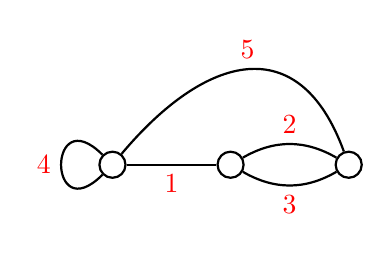
\begin{tikzpicture}[node distance={15mm}, thick, main/.style = {draw, circle}]
\node[main] (1){};
\node[main] (2) [right of=1]{};
\node[main] (3) [right of=2]{};
\draw (1) -- node[midway,below,pos=0.5] {\textcolor{red}{1}} (2);
\draw (1) to [out=50,in=110,looseness=1.5] node[midway,above,pos=0.5] {\textcolor{red}{5}} (3);
\draw (1) to [out=135,in=225,looseness=10] node[midway,left,pos=0.5] {\textcolor{red}{4}} (1);
\draw (2) to [out=30,in=150,looseness=1] node[midway,above,pos=0.5] {\textcolor{red}{2}} (3);
\draw (2) to [out=330,in=210,looseness=1] node[midway,below,pos=0.5] {\textcolor{red}{3}} (3);
\end{tikzpicture}
\end{figure}

Here, $E$ is the set of edges. \pause The cycles of this graph are $ \{\textcolor{red}{1},\textcolor{red}{2},\textcolor{red}{5}\}, \{\textcolor{red}{1},\textcolor{red}{3},\textcolor{red}{5}\}, \{\textcolor{red}{2},\textcolor{red}{3}\}, \{ \textcolor{red}{4} \}$. The independent sets are just the sets of edges that do not contain a cycle.
\end{frame}

\begin{frame}[fragile]{Independent Sets, Bases}
Our setup - finite set $E$, collection of its subsets $\mathcal{I}$ satisfying: \pause
\begin{enumerate}
\item $\emptyset \in \mathcal{I}.$
\pause
\item If $I \in \mathcal{I}$ and $J \subset I$, then $J \in \mathcal{I}$.
\pause
\item If $J, I \in \mathcal{I}$ and $|J| < |I|$, then there is $e \in I - J$ such that $J \cup e \in \mathcal{I}$.
\end{enumerate}

\pause
\begin{center}
    

\begin{tikzpicture}

\matrix (a) [matrix of math nodes, column sep=0.6cm, row sep=0.6cm,]{
 & & &\textcolor{cyan}{
1234} & & & &\\
 \textcolor{cyan}{
123}& &\textcolor{cyan}{
124} & &\textcolor{cyan}{
134} &  & \textcolor{cyan}{
234}  \\
\textcolor{red}{12} & \textcolor{cyan}{13} & \textcolor{cyan}{14} & & \textcolor{red}{23} & \textcolor{cyan}{
24} & \textcolor{cyan}{
34} \\
\textcolor{orange}{1}& &\textcolor{orange}{2} & & \textcolor{orange}{3}& & \textcolor{cyan}{4} \\
& & & \textcolor{orange}{\emptyset} &  & & \\
&&&&&& \\};



\foreach \i/\j in {1-4/2-1, 1-4/2-3, 1-4/2-5, 1-4/2-7, 2-1/3-1, 2-1/3-2, 2-1/3-5, 2-3/3-1, 2-3/3-3, 2-3/3-6, 2-5/3-2, 2-5/3-3, 2-5/3-7, 2-7/3-5, 2-7/3-6, 2-7/3-7, 3-1/4-1, 3-1/4-3, 3-2/4-1, 3-2/4-5, 3-3/4-1, 3-3/4-7, 3-5/4-3, 3-5/4-5, 3-6/4-3, 3-6/4-7, 3-7/4-7, 3-7/4-5, 4-1/5-4, 4-3/5-4, 4-5/5-4, 4-7/5-4}
\draw[double, line width = 0.005mm, color = brown] (a-\i) -- (a-\j);

\node[draw] at (0, -2.5){\small \textcolor{orange}{Independent set}, \textcolor{red}{Basis}, \textcolor{cyan}{Dependent set}}




\end{tikzpicture}

\end{center}


\end{frame}

\begin{frame}[fragile]{Circuits --- motivation}

\begin{itemize}
 \item  Cycles are central to graph theory.
 \pause
 \item Intuitively, spanning trees and (the absence) of cycles are intimately connected.
 \pause
 \item     It turns out this idea can be used to describe general matroids using a generalized notion of cycles --- \textit{Circuits}.
\end{itemize}

\pause
\begin{center}
    

\begin{tikzpicture}

\matrix (a) [matrix of math nodes, column sep=0.6cm, row sep=0.6cm,]{
 & & &\textcolor{cyan}{
1234} & & & &\\
 \textcolor{cyan}{
123}& &\textcolor{cyan}{
124} & &\textcolor{cyan}{
134} &  & \textcolor{cyan}{
234}  \\
\textcolor{red}{12} & \textcolor{blue}{13} & \textcolor{cyan}{14} & & \textcolor{red}{23} & \textcolor{cyan}{
24} & \textcolor{cyan}{
34} \\
\textcolor{orange}{1}& &\textcolor{orange}{2} & & \textcolor{orange}{3}& & \textcolor{blue}{4} \\
& & & \textcolor{orange}{\emptyset} &  & & \\
&&&&&& \\};



\foreach \i/\j in {1-4/2-1, 1-4/2-3, 1-4/2-5, 1-4/2-7, 2-1/3-1, 2-1/3-2, 2-1/3-5, 2-3/3-1, 2-3/3-3, 2-3/3-6, 2-5/3-2, 2-5/3-3, 2-5/3-7, 2-7/3-5, 2-7/3-6, 2-7/3-7, 3-1/4-1, 3-1/4-3, 3-2/4-1, 3-2/4-5, 3-3/4-1, 3-3/4-7, 3-5/4-3, 3-5/4-5, 3-6/4-3, 3-6/4-7, 3-7/4-7, 3-7/4-5, 4-1/5-4, 4-3/5-4, 4-5/5-4, 4-7/5-4}
\draw[double, line width = 0.005mm, color = brown] (a-\i) -- (a-\j);

\node[draw] at (0, -2.5){\small \textcolor{orange}{Independent set}, \textcolor{red}{Basis}, \textcolor{blue}{Circuit}, \textcolor{cyan}{Dependent set}}



\end{tikzpicture}

\end{center}


\end{frame}


\begin{frame}{Circuits --- Definition}
    \begin{itemize}
        \item \textit{Circuits} are minimal dependent sets
        \pause
        \item We can formally define a matroid given its ground set $E$ and a set of circuits $\mathcal C$:
    \end{itemize}
        \pause
            \begin{enumerate}
                \item $\emptyset \not\in \mathcal C$ (the empty set cannot be dependent)
                \pause
                \item If $C_1, C_2 \in \mathcal C$ and $C_1 \subseteq C_2$ then $C_1 = C_2$ (otherwise $C_2$ would clearly not be minimal)
                \pause
                \item If $C_1, C_2 \in \mathcal C$ are distinct circuits and $e \in C_1 \cap C_2$ then a circuit $C_3 \in \mathcal C$ exists with $C_3 \subseteq (C_1 \cup C_2) - e$
            \end{enumerate}



\pause


                  \begin{figure}
\begin{subfigure}[h]{0.2\textwidth}
  \caption{Graph}
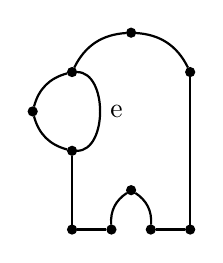
\begin{tikzpicture}[node distance={10mm}, thick, main/.style = {draw,circle,fill,inner sep=1pt}] 
  \node[main] (1) at (0,0) {}; 
  \node[main] (3) at (-0.5,0.5) {}; 
  \node[main] (4) at (0, 1) {}; 
  \node[main] (5) at (0, -1) {}; 
  \node[main] (6) at (1.5, -1) {}; 
  \node[main] (7) at (0.75, 1.5) {}; 
  \node[main] (8) at (1.5, 1) {}; 
  \node[main] (9) at (0.5, -1) {}; 
  \node[main] (10) at (1, -1) {}; 
  \node[main] (11) at (0.75, -0.5) {}; 
  \draw (1) to [bend left] (3);
  \draw (1) to [bend right=90]
node[midway, right] {e} (4) ;
  \draw (3) to [bend left] (4);
  \draw (4) to [bend left] (7);
  \draw (7) to [bend left] (8);
  \draw (8) to (6);
  \draw (5) to (9);
  \draw (6) to (10);
  \draw (9) to [bend left] (11);
  \draw (10) to [bend right] (11);
  \draw (5) to (1);
\end{tikzpicture} 
\end{subfigure}
\pause
\begin{subfigure}[h]{0.2\textwidth}
  \caption{C _1 }
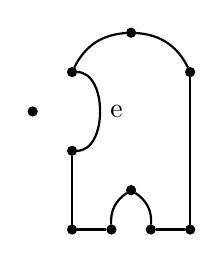
\begin{tikzpicture}[node distance={10mm}, thick, main/.style = {draw,circle,fill,inner sep=1pt}] 
  \node[main] (1) at (0,0) {}; 
  \node[main] (3) at (-0.5,0.5) {}; 
  \node[main] (4) at (0, 1) {}; 
  \node[main] (5) at (0, -1) {}; 
  \node[main] (6) at (1.5, -1) {}; 
  \node[main] (7) at (0.75, 1.5) {}; 
  \node[main] (8) at (1.5, 1) {}; 
  \node[main] (9) at (0.5, -1) {}; 
  \node[main] (10) at (1, -1) {}; 
  \node[main] (11) at (0.75, -0.5) {}; 
  \draw (1) to [bend right=90]
node[midway, right] {e} (4) ;
  \draw (4) to [bend left] (7);
  \draw (7) to [bend left] (8);
  \draw (8) to (6);
  \draw (5) to (9);
  \draw (6) to (10);
  \draw (9) to [bend left] (11);
  \draw (10) to [bend right] (11);
  \draw (5) to (1);
\end{tikzpicture} 
\end{subfigure}
\pause
\begin{subfigure}[h]{0.2\textwidth}
  \caption{C _2 }
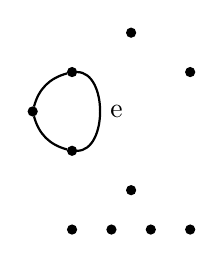
\begin{tikzpicture}[node distance={10mm}, thick, main/.style = {draw,circle,fill,inner sep=1pt}] 
  \node[main] (1) at (0,0) {}; 
  \node[main] (3) at (-0.5,0.5) {}; 
  \node[main] (4) at (0, 1) {}; 
  \node[main] (5) at (0, -1) {}; 
  \node[main] (6) at (1.5, -1) {}; 
  \node[main] (7) at (0.75, 1.5) {}; 
  \node[main] (8) at (1.5, 1) {}; 
  \node[main] (9) at (0.5, -1) {}; 
  \node[main] (10) at (1, -1) {}; 
  \node[main] (11) at (0.75, -0.5) {}; 
  \draw (1) to [bend left] (3);
  \draw (1) to [bend right=90]
node[midway, right] {e} (4) ;
  \draw (3) to [bend left] (4);
\end{tikzpicture} 
\end{subfigure}
\pause
\begin{subfigure}[h]{0.2\textwidth}
  \caption{C _3 } 
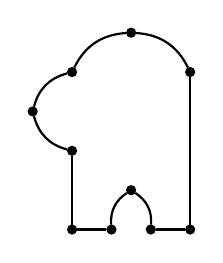
\begin{tikzpicture}[node distance={10mm}, thick, main/.style = {draw,circle,fill,inner sep=1pt}] 
  \node[main] (1) at (0,0) {}; 
  \node[main] (3) at (-0.5,0.5) {}; 
  \node[main] (4) at (0, 1) {}; 
  \node[main] (5) at (0, -1) {}; 
  \node[main] (6) at (1.5, -1) {}; 
  \node[main] (7) at (0.75, 1.5) {}; 
  \node[main] (8) at (1.5, 1) {}; 
  \node[main] (9) at (0.5, -1) {}; 
  \node[main] (10) at (1, -1) {}; 
  \node[main] (11) at (0.75, -0.5) {}; 
  \draw (1) to [bend left] (3);
  \draw (3) to [bend left] (4);
  \draw (4) to [bend left] (7);
  \draw (7) to [bend left] (8);
  \draw (8) to (6);
  \draw (5) to (9);
  \draw (6) to (10);
  \draw (9) to [bend left] (11);
  \draw (10) to [bend right] (11);
  \draw (5) to (1);
\end{tikzpicture} 
\end{subfigure}
                  \end{figure}

\end{frame}

\begin{frame}{Rank Function, Closure}
    \begin{itemize}
        \item The notion of \textit{rank} from linear algebra can also be generalized to arbitrary matroids.\pause The rank of a set $S$, denoted r($S$), measures the size of the largest independent sets contained in $S$. For example, the rank of the ground set $E$ is the size of a basis of the matroid (since all bases are of the same size).
\pause
        \item The closure of a set $S$, denoted $\cl(S)$, is the maximal superset of $S$ with equal rank. In other words:
        \pause
        \begin{align*} 
        \cl(S) = \{x\in E : \rank(S\cup x)=\rank(S)\} .\end{align*}
    \end{itemize}
\end{frame}

\begin{frame}{Rank Function, Closure --- examples}
  \begin{enumerate}[<+->]
    \item Graphic matroids:
      \begin{itemize}
        \item the rank function measures the size of the spanning forest.
        \item the closure is the maximal superset one can obtain by only adding edges when they introduce cycles.
      \end{itemize}

    \item Vector matroids: 
      \begin{itemize}
        \item the rank function measures the rank of the submatrix, so the dimention of the span.
        \item the closure operator constructs the span, intersected with $E$.
      \end{itemize}

    \end{enumerate}
\end{frame}
\begin{frame}{Rank Function, Closure Operator --- worked example}
    Consider the matroid induced by the graph $G$, and the set $S$ defined below. 
      \begin{itemize}
        \item<3-> $U$ is a spanning forest (we removed $c$ to get rid of a cycle)
        \item<4-> The rank is the size of the spanning forest, i.e. $\rank(S) = |U| = 11$.
        \item<5-> The only edges which introduce cycles when added to $S$ are $a$ and $b$, so $\cl(S) = S + a + b$.
      \end{itemize}
                  \begin{figure}
\onslide<1->{\begin{subfigure}[h]{0.2\textwidth}
  \caption{$G$}
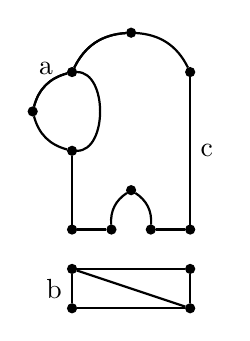
\begin{tikzpicture}[node distance={10mm}, thick, main/.style = {draw,circle,fill,inner sep=1pt}] 
  \node[main] (1) at (0,0) {}; 
  \node[main] (3) at (-0.5,0.5) {}; 
  \node[main] (4) at (0, 1) {}; 
  \node[main] (5) at (0, -1) {}; 
  \node[main] (6) at (1.5, -1) {}; 
  \node[main] (7) at (0.75, 1.5) {}; 
  \node[main] (8) at (1.5, 1) {}; 
  \node[main] (9) at (0.5, -1) {}; 
  \node[main] (10) at (1, -1) {}; 
  \node[main] (11) at (0.75, -0.5) {}; 
  \node[main] (12) at (0, -1.5) {}; 
  \node[main] (13) at (1.5, -1.5) {}; 
  \node[main] (14) at (1.5, -2) {}; 
  \node[main] (15) at (0, -2) {}; 
  \draw (1) to [bend left] (3);
  \draw (4) to [bend left] (7);
  \draw (1) to [bend right=90] (4);
  \draw (3) to [bend left]
node[midway, above] {a} (4) ;
  \draw (3) to [bend left] (4);
  \draw (4) to [bend left] (7);
  \draw (7) to [bend left] (8);
  \draw (6) to node[midway, right] {c} (8) ;
  \draw (5) to (9);
  \draw (6) to (10);
  \draw (9) to [bend left] (11);
  \draw (10) to [bend right] (11);
  \draw (5) to (1);
  \draw (12) to (13);
  \draw (13) to (14);
  \draw (15) to (14);
  \draw (12) to
node[midway, left] {b} (15) ;
  \draw (12) to (14);
\end{tikzpicture} 
\end{subfigure}}
\onslide<2->{\begin{subfigure}[h]{0.2\textwidth}
  \caption{$S$}
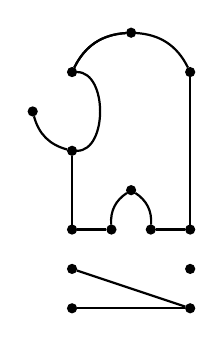
\begin{tikzpicture}[node distance={10mm}, thick, main/.style = {draw,circle,fill,inner sep=1pt}] 
  \node[main] (1) at (0,0) {}; 
  \node[main] (3) at (-0.5,0.5) {}; 
  \node[main] (4) at (0, 1) {}; 
  \node[main] (5) at (0, -1) {}; 
  \node[main] (6) at (1.5, -1) {}; 
  \node[main] (7) at (0.75, 1.5) {}; 
  \node[main] (8) at (1.5, 1) {}; 
  \node[main] (9) at (0.5, -1) {}; 
  \node[main] (10) at (1, -1) {}; 
  \node[main] (11) at (0.75, -0.5) {}; 
  \node[main] (12) at (0, -1.5) {}; 
  \node[main] (13) at (1.5, -1.5) {}; 
  \node[main] (14) at (1.5, -2) {}; 
  \node[main] (15) at (0, -2) {}; 
  \draw (1) to [bend left] (3);
  \draw (1) to [bend right=90] (4);
  \draw (4) to [bend left] (7);
  \draw (4) to [bend left] (7);
  \draw (7) to [bend left] (8);
  \draw (8) to (6);
  \draw (5) to (9);
  \draw (6) to (10);
  \draw (9) to [bend left] (11);
  \draw (10) to [bend right] (11);
  \draw (5) to (1);
  \draw (14) to (15);
  \draw (12) to (14);
\end{tikzpicture} 
\end{subfigure}}
\onslide<3->{\begin{subfigure}[h]{0.2\textwidth}
  \caption{$U$}
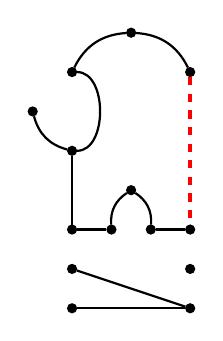
\begin{tikzpicture}[node distance={10mm}, thick, main/.style = {draw,circle,fill,inner sep=1pt}] 
  \node[main] (1) at (0,0) {}; 
  \node[main] (3) at (-0.5,0.5) {}; 
  \node[main] (4) at (0, 1) {}; 
  \node[main] (5) at (0, -1) {}; 
  \node[main] (6) at (1.5, -1) {}; 
  \node[main] (7) at (0.75, 1.5) {}; 
  \node[main] (8) at (1.5, 1) {}; 
  \node[main] (9) at (0.5, -1) {}; 
  \node[main] (10) at (1, -1) {}; 
  \node[main] (11) at (0.75, -0.5) {}; 
  \node[main] (12) at (0, -1.5) {}; 
  \node[main] (13) at (1.5, -1.5) {}; 
  \node[main] (14) at (1.5, -2) {}; 
  \node[main] (15) at (0, -2) {}; 
  \draw (1) to [bend right=90] (4);
  \draw (1) to [bend left] (3);
  \draw (4) to [bend left] (7);
  \draw (7) to [bend left] (8);
  \draw (5) to (9);
  \draw (6) to (10);
  \draw[dashed, ultra thick, red] (8) to (6);
  \draw (9) to [bend left] (11);
  \draw (10) to [bend right] (11);
  \draw (5) to (1);
  \draw (14) to (15);
  \draw (12) to (14);
\end{tikzpicture} 
\end{subfigure}}
\onslide<5->{\begin{subfigure}[h]{0.2\textwidth}
  \caption{$\cl(S)$} 
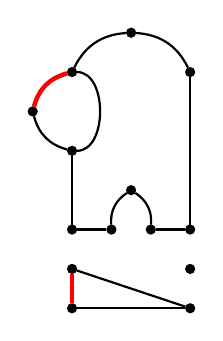
\begin{tikzpicture}[node distance={10mm}, thick, main/.style = {draw,circle,fill,inner sep=1pt}] 
  \node[main] (1) at (0,0) {}; 
  \node[main] (3) at (-0.5,0.5) {}; 
  \node[main] (4) at (0, 1) {}; 
  \node[main] (5) at (0, -1) {}; 
  \node[main] (6) at (1.5, -1) {}; 
  \node[main] (7) at (0.75, 1.5) {}; 
  \node[main] (8) at (1.5, 1) {}; 
  \node[main] (9) at (0.5, -1) {}; 
  \node[main] (10) at (1, -1) {}; 
  \node[main] (11) at (0.75, -0.5) {}; 
  \node[main] (12) at (0, -1.5) {}; 
  \node[main] (13) at (1.5, -1.5) {}; 
  \node[main] (14) at (1.5, -2) {}; 
  \node[main] (15) at (0, -2) {}; 
  \draw (1) to [bend left] (3);
  \draw (1) to [bend right=90] (4);
  \draw[ultra thick, red] (3) to [bend left] (4);
  \draw (4) to [bend left] (7);
  \draw (7) to [bend left] (8);
  \draw (8) to (6);
  \draw (5) to (9);
  \draw (6) to (10);
  \draw (9) to [bend left] (11);
  \draw (10) to [bend right] (11);
  \draw (5) to (1);
  \draw (14) to (15);
  \draw[ultra thick, red] (15) to  (12);
  \draw (12) to (14);
\end{tikzpicture} 
\end{subfigure}}
                  \end{figure}
\end{frame}



\begin{frame}[fragile]{Duality - Definition}
       Given a matroid $M$, the dual of $M$ is a matroid denoted by $M^*$ having the same ground set $E$, such that the bases of $M^*$ are precisely the complements of bases of $M$. \pause Formally:
       
    \begin{itemize}
        \item let $M$ be a matroid on $E$ with $\mathcal{B}$ as its collection of bases, and: 
        \begin{align*} 
        \mathcal B^*(M) =  \{E(M) - B:B\in \mathcal B(M)\}.
        \end{align*}
        
    \item Then the dual matroid $M^*$ is a matroid having $\mathcal{B}^*(M)$ as its collection of bases.
    \end{itemize}
\pause
\begin{center}
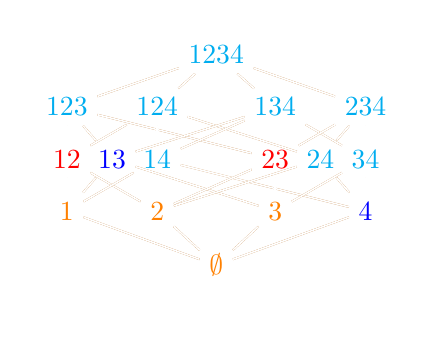
\begin{tikzpicture}

\matrix (a) [matrix of math nodes, column sep=-0.1cm, row sep=0.2cm,]{
 & & &\textcolor{cyan}{
1234} & & & &\\
 \textcolor{cyan}{
123}& &\textcolor{cyan}{
124} & &\textcolor{cyan}{
134} &  & \textcolor{cyan}{
234}  \\
\textcolor{red}{12} & \textcolor{blue}{13} & \textcolor{cyan}{14} & & \textcolor{red}{23} & \textcolor{cyan}{
24} & \textcolor{cyan}{
34} \\
\textcolor{orange}{1}& &\textcolor{orange}{2} & & \textcolor{orange}{3}& & \textcolor{blue}{4} \\
& & & \textcolor{orange}{\emptyset} &  & & \\
&&&&&& \\};

\foreach \i/\j in {1-4/2-1, 1-4/2-3, 1-4/2-5, 1-4/2-7, 2-1/3-1, 2-1/3-2, 2-1/3-5, 2-3/3-1, 2-3/3-3, 2-3/3-6, 2-5/3-2, 2-5/3-3, 2-5/3-7, 2-7/3-5, 2-7/3-6, 2-7/3-7, 3-1/4-1, 3-1/4-3, 3-2/4-1, 3-2/4-5, 3-3/4-1, 3-3/4-7, 3-5/4-3, 3-5/4-5, 3-6/4-3, 3-6/4-7, 3-7/4-7, 3-7/4-5, 4-1/5-4, 4-3/5-4, 4-5/5-4, 4-7/5-4}
\draw[double, line width = 0.005mm, color = brown] (a-\i) -- (a-\j);

\end{tikzpicture}
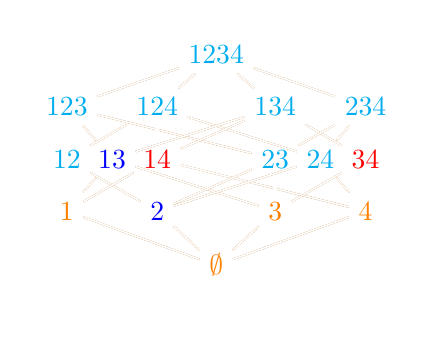
\begin{tikzpicture}

\matrix (a) [matrix of math nodes, column sep=-0.1cm, row sep=0.2cm,]{
 & & &\textcolor{cyan}{
1234} & & & &\\
 \textcolor{cyan}{
123}& &\textcolor{cyan}{
124} & &\textcolor{cyan}{
134} &  & \textcolor{cyan}{
234}  \\
\textcolor{cyan}{12} & \textcolor{blue}{13} & \textcolor{red}{14} & & \textcolor{cyan}{23} & \textcolor{cyan}{
24} & \textcolor{red}{
34} \\
\textcolor{orange}{1}& &\textcolor{blue}{2} & & \textcolor{orange}{3}& & \textcolor{orange}{4} \\
& & & \textcolor{orange}{\emptyset} &  & & \\
&&&&&& \\};

\foreach \i/\j in {1-4/2-1, 1-4/2-3, 1-4/2-5, 1-4/2-7, 2-1/3-1, 2-1/3-2, 2-1/3-5, 2-3/3-1, 2-3/3-3, 2-3/3-6, 2-5/3-2, 2-5/3-3, 2-5/3-7, 2-7/3-5, 2-7/3-6, 2-7/3-7, 3-1/4-1, 3-1/4-3, 3-2/4-1, 3-2/4-5, 3-3/4-1, 3-3/4-7, 3-5/4-3, 3-5/4-5, 3-6/4-3, 3-6/4-7, 3-7/4-7, 3-7/4-5, 4-1/5-4, 4-3/5-4, 4-5/5-4, 4-7/5-4}
\draw[double, line width = 0.005mm, color = brown] (a-\i) -- (a-\j);

\end{tikzpicture}
\end{center}

\begin{center}
\begin{tikzpicture}
\node[draw] at (0, -2.5){\small \textcolor{orange}{Independent set}, \textcolor{red}{Basis}, \textcolor{blue}{Circuit}, \textcolor{cyan}{Dependent set}}
\end{tikzpicture}
\end{center}

\end{frame}

\begin{frame}{Duality - Properties}
Notation: The bases of $M^*$ are called cobases of $M$
    \begin{itemize}[<+->]
        \item $(M^*)^* = M$
        \item Let $M$ be a matroid in a set $E$ and suppose $X \subseteq E$. Then
            \begin{enumerate}
                \item $X$ is \textit{independent} if and only if $E-X$ is \textit{cospanning}.
                \item $X$ is \textit{spanning} if and only if $E-X$ is \textit{coindependent}.
            \end{enumerate}
        \item If \textit{M} is \textit{representable} over the field \textit{F}, then \textit{M*} is also representable over \textit{F}. 
        \item $r(M) + r^*(M) = |E(M)| = |E(M^*)|$
        \item $r^*(X) = r(E - X) + |X| - r(M)$
    \end{itemize}    
\end{frame}

%%%

\begin{frame}{Duality - Examples}
    Example 1:
    Let us consider the bipartite graph $K_{3,3}$. 
    \pause
    \begin{figure}
    \centering
    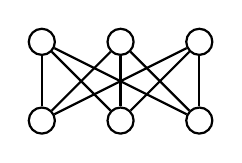
\begin{tikzpicture}[node distance={10mm}, thick, main/.style = {draw, circle}] 
        \node[main] (1) {}; 
        \node[main] (2) [below of=1] {}; 
        \node[main] (3) [right of=1] {}; 
        \node[main] (4) [below of=3] {}; 
        \node[main] (5) [right of=3] {}; 
        \node[main] (6) [below of=5] {}; 
        \draw (1) to (2); 
        \draw (1) to (4);
        \draw (1) to (6); 
        \draw (3) to (2);
        \draw (3) to (4); 
        \draw (3) to (6);
        \draw (5) to (2); 
        \draw (5) to (4);
        \draw (5) to (6);
        \end{tikzpicture}
    \end{figure}
    We can see it has 9 edges, so the ground set is $E=\{1,2,3, \dots, 9\} $.
    \pause
    \begin{figure}
    The matrix associated to the matroid $M(K_{3,3})$ is the following:
    $$B = \begin{bmatrix}
    1 & 0 & 0 & 0 & 0 & 1 & 0 & 0 & 1\\
    0 & 1 & 0 & 0 & 0 & 1 & 1 & 0 & 1\\
    0 & 0 & 1 & 0 & 0 & 1 & 1 & 1 & 1\\
    0 & 0 & 0 & 1 & 0 & 0 & 1 & 1 & 1\\
    0 & 0 & 0 & 0 & 1 & 0 & 0 & 1 & 1\\
    \end{bmatrix}$$
    \end{figure}
\end{frame}

\begin{frame}{Duality - Examples}

\begin{theorem} Let M be the vector matroid of the matrix $[I_r|D]$ where the columns of this matrix are labelled, in order, $e_1, e_2,...,e_n$ and $1 \leq r< n$. \pause Then $M^*$ is the vector matroid of $[-D^T|I_{n-r}]$ where its columns are also labelled $e_1, e_2,...,e_n$ in that order.
\end{theorem}
\pause
So, the dual matroid $M^*(K_{3,3})$ is represented by the following matrix:
$$B^* = \begin{bmatrix}
1 & 1 & 1 & 0 & 0 & 1 & 0 & 0 & 0\\
0 & 1 & 1 & 1 & 0 & 0 & 1 & 0 & 0\\
0 & 0 & 1 & 1 & 1 & 0 & 0 & 1 & 0\\
1 & 1 & 1 & 1 & 1 & 0 & 0 & 0 & 1\\
\end{bmatrix}$$

\end{frame}

\begin{frame}{Duality - Examples}
    So we have, 
\begin{figure}
        $$B=\!\!\!\begin{bmatrix}
    1 & 0 & 0 & 0 & 0 & 1 & 0 & 0 & 1\\
    0 & 1 & 0 & 0 & 0 & 1 & 1 & 0 & 1\\
    0 & 0 & 1 & 0 & 0 & 1 & 1 & 1 & 1\\
    0 & 0 & 0 & 1 & 0 & 0 & 1 & 1 & 1\\
    0 & 0 & 0 & 0 & 1 & 0 & 0 & 1 & 1\\
    \end{bmatrix}
  %
  B^*=\!\!\!\begin{bmatrix} 
1 & 1 & 1 & 0 & 0 & 1 & 0 & 0 & 0\\
0 & 1 & 1 & 1 & 0 & 0 & 1 & 0 & 0\\
0 & 0 & 1 & 1 & 1 & 0 & 0 & 1 & 0\\
1 & 1 & 1 & 1 & 1 & 0 & 0 & 0 & 1\\
\end{bmatrix}$$
\end{figure}
\pause
Where, $r(M) = 5$ and $r^*(M)=4$, and $|E(M)|=9$.
Hence, we see that $r(M) + r^*(M) = |E(M)|$ holds.

\pause Also, in this example, both matroids are vector matroids over the field $\mathbb{F}_2$. 
\pause However, although $M(K_{3,3})$ is a graphic matroid, its dual, $M^*(K_{3,3})$ is not graphic. This results points to the following: \pause
\begin{theorem}
    \item  The dual of a graphic matroid is itself graphic if and only if the underlying graph is planar.
\end{theorem}

\end{frame}

% every breath you take every
% ^^ what?
\begin{frame}{To summarize}
\pause
\begin{itemize}[<+->]
    \item We abstracted linear independence with three axioms.
    \item This abstract independence turns out to have connections to other fields too, like graph theory.
    \item Each matroid has circuits, bases, rank function and closure operator, each with their unique properties that determine them from the reverse direction.
    \item Every matroid has an "opposite matroid" called its dual, that is formed using the complements of the bases of the original matroid.
\end{itemize}

\end{frame}


\begin{frame}{References}
\begin{itemize}[<+->]
    \item  J. G. Oxley. Matroid theory. Oxford Science Publications. Oxford University Press, USA, 1993.  
    \item G. Gordon and J. McNulty. Matroids: A geometric introduction. Cambridge University Press, 2021.

\end{itemize}
  
\end{frame}



\begin{frame}{}

\begin{center}
\huge Thank You!
\end{center}
    
\end{frame}


For can now give and example for the concepts given until know.

\textit{Example:}




Now, we will formulate another important point, the so called, orthogonality, which refers to the link between circuits and cocircuits. 

\textit{Proposition:} For a given matroid M, let C be a circuit and C* be a cocircuit. Then,  
$|C \cap C*| \neq 1$.

\begin{proof}
    We will prove this by contradiction. Suppose $C \cap C* = \{x\}$, for some $x \in E$, this is, there exists and element in the intersection such that the cardinality will be 1. Now consider the hyperplane $H=E-C^*$, and recall that the closure $cl(H)=H$. We can onserve that by the way in which it is defined if $x\in C^*$, then $x\notin H$, but $C-x\subseteq H$. Moreover, we have that $x\in cl(C-x)$ hence $x\in cl(H)=H$. Then $x\notin C^*$, which is a contradiction. So, $C \cap C* \neq \{x\}$, which implies $|C \cap C*| \neq 1$.
\end{proof}


\end{document}
